%% Los cap'itulos inician con \chapter{T'itulo}, estos aparecen numerados y
%% se incluyen en el 'indice general.
%%
%% Recuerda que aqu'i ya puedes escribir acentos como: 'a, 'e, 'i, etc.
%% La letra n con tilde es: 'n.

\chapter{Propuesta}
Se propone un abordaje basado en la t\'ecnicas de procesamiento de imagenes que servir\'an para implementar el sistema de visi\'on global, el cual tendr\'a como salida la posici\'on y orientaci\'on actual en cada frame del robot. Luego de este proceso se utilizar\'a una red neuronal  que aprender\'a de los estados y las posiciones y predecir\'a los siguientes estados para hacerle el seguimiento. El esquema se presenta en la figura 4.1: \\
	\begin{figure}
	\centering
	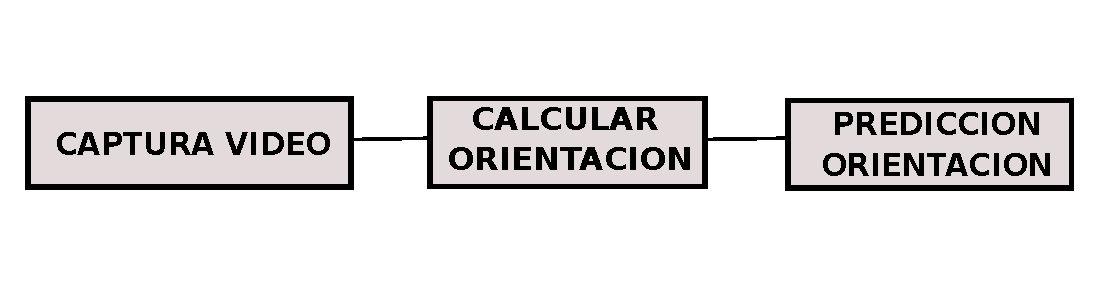
\includegraphics[width=2.5in]{esquema.pdf}
	
	\caption{Esquema del Sistema}
	\label{fig_mar}
\end{figure}
\section{Sistema de Visi\'on}
Para esto utilizamos marcas encima de los robots, las cuales nos dan mas facilidades para realizar la identificaci\'on de cada robot como se muestra en la Figura 4.2.
	\begin{figure}
	\centering
	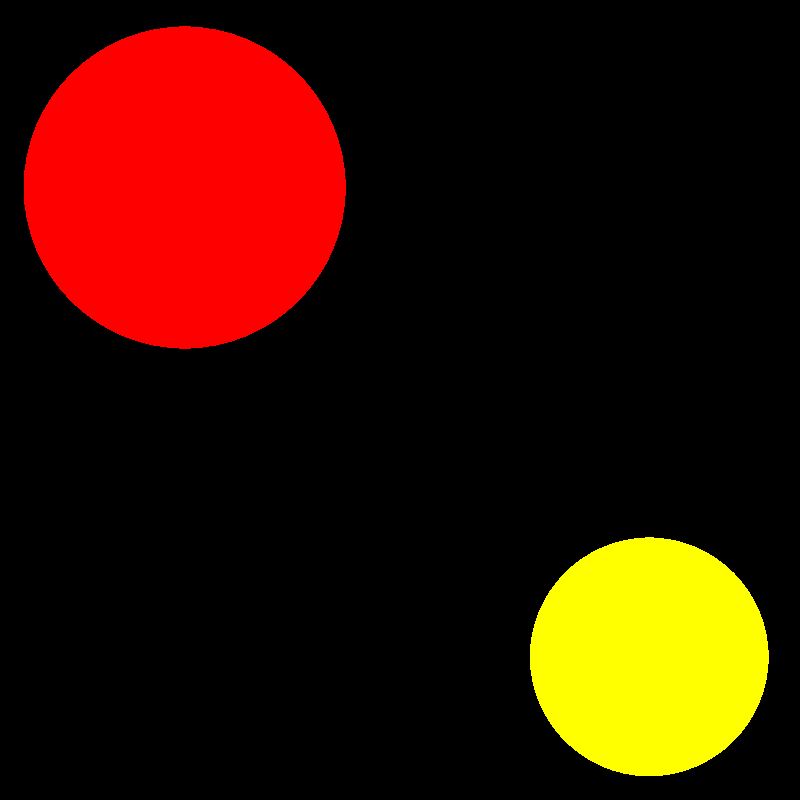
\includegraphics[width=2.5in]{imagen1.pdf}
	
	\caption{Marcas en cada robot}
	\label{fig_mar}
\end{figure}
En el sistema de vision proponemos utilizar los m\'etodos de el filtro de Gauss y la transformada de Hough. Para realizar esto utilizamos la libreria de OpenCv, la cual nos da soporte para primero aplicar un filtro de gauss para eliminar el ruido en nuestra imagen, luego convertimos nuestra imagen a la escala de grises, y finalmente aplicamos la transformada de Hough para obtener los c\'irculos en la imagen, cuyos centros tambien son hallados.\\
Una vez hallados los centros y radios de cada circulo procedemos a realizar el calculo de la ubicacion de nuestro robot, el cual utilizara unos circulos marcados como se muestra en la Fig  \ref{fig_cir}. Entonces como tenemos dos circulos de ubicacion conocida procedemos a aplicar el metodo  que nos dice que la posicion basado en esos dos circulos estara en el punto medio de la recta que une los dos centros  $c_i$ y $c_j$ de los dos circulos \cite{kelson_glo}. Entonces aplicamos punto medio entre los dos centros de los circulos:
\begin{equation}
x=\frac{x_1+y_2}{2} \qquad; y=\frac{y_1+y_2}{{2}}
\end{equation}

Una vez hallada la posicion actual del robot procedemos a hallar la orientacion con respecto al eje inicial del la imagen, de la misma forma utilizamos un metodo ya utilizado anterioremente,  el cual consiste en comparar los puntos centrales y con su tangente hallar la orientacion (angulo)\cite{kelson_glo}. El angulo $\theta$ de orientacion seria dado por:
\begin{equation}
\theta=arctan(\frac{y_1-y_2}{x_1-x_2} )
\end{equation}

\begin{figure}
\centering
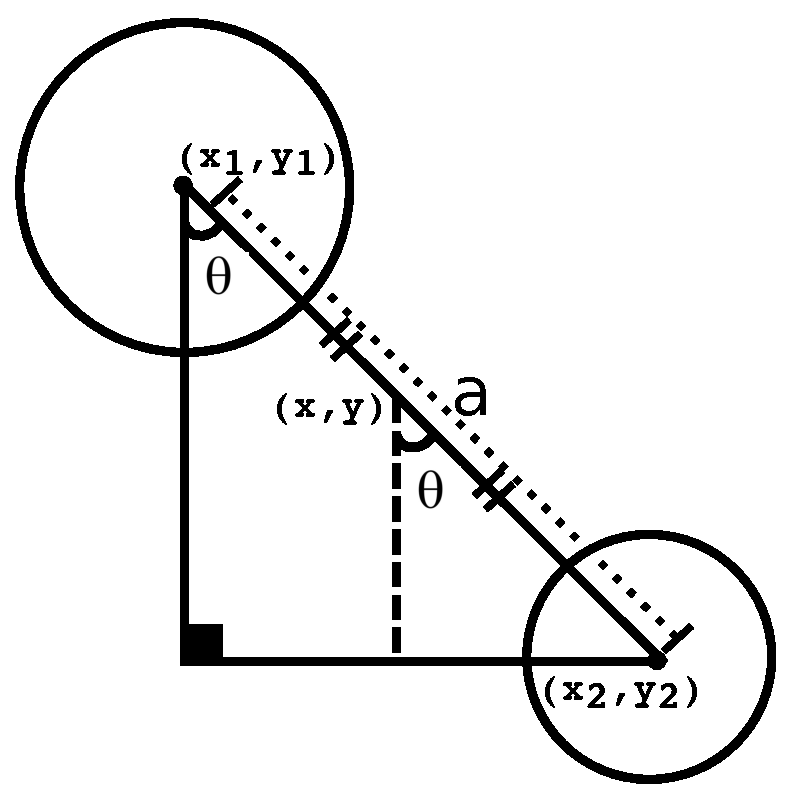
\includegraphics[width=2.5in]{imagen2.pdf}
\caption{C\'alculo de la posici\'on}
\label{fig_cir}
\end{figure}
Asi ya tenemos la posici\'on actual en cada frame y la orientaci\'on que sigue cada robot, y estamos preparados para darle estos par\'ametros a la red neuronal  y se pueda predecir su siguiente posici\'on.


\section{Seguimiento del Objeto}
Para realizar el seguimiento utilizaremos una Red Neuronal de Base Radial, la cual consiste en una red con una  capa de unidades ocultas, conectadas a las entradas y una neurona de salida, con transmicion directa (feedforward), donde las funciones de transferencia entre nodos (o neurones) son funciones simetricas radialmente. La estructura de la Red RBF es similar a la de la figura 4.4.
\begin{figure}
\centering
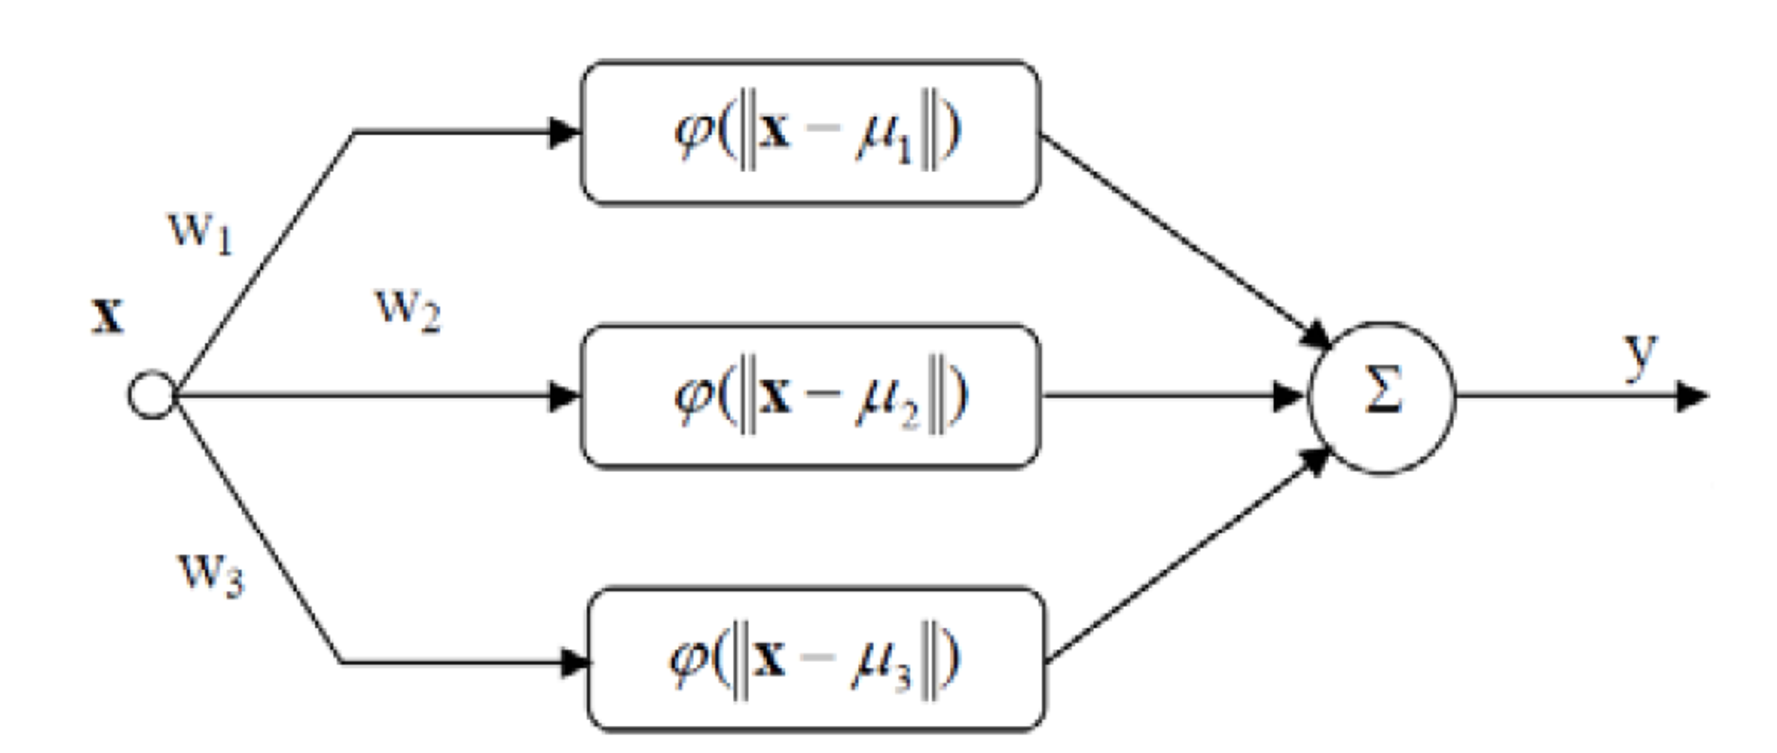
\includegraphics[width=2.5in]{RBF.pdf}
\caption{Red Neuronal de Base Radial }
\label{fig_cir}
\end{figure}

La salida para una red RBF, viene dada por: 
\[
\sum_{i=1}^{M}W_{i}\varphi(||x-\mu_i||)
\]

Donde $\varphi$ representa la funcion simetrica radialmente.
El aprendizaje en una red RBF debe ser basado en el minimizar el error, bajo la siguiente ecuacion.
\[
\sum_{p=1}^{P}(z_p-y_p)
\]
Donde $z_p$ es el valor conocido como salida, en nuestro caso la orientacion en el tiempo $t+1$, y $y_p$ es el valor de la salida de la red.\\
A esta igualdad le aplicamos el metodo de gradiente y la funcion Gaussiana,  luego de realizar los reemplazos correspondientes, nos queda que la variacion  del peso $w_i$ es como en la figura 4.5:\\
\begin{figure}
\centering
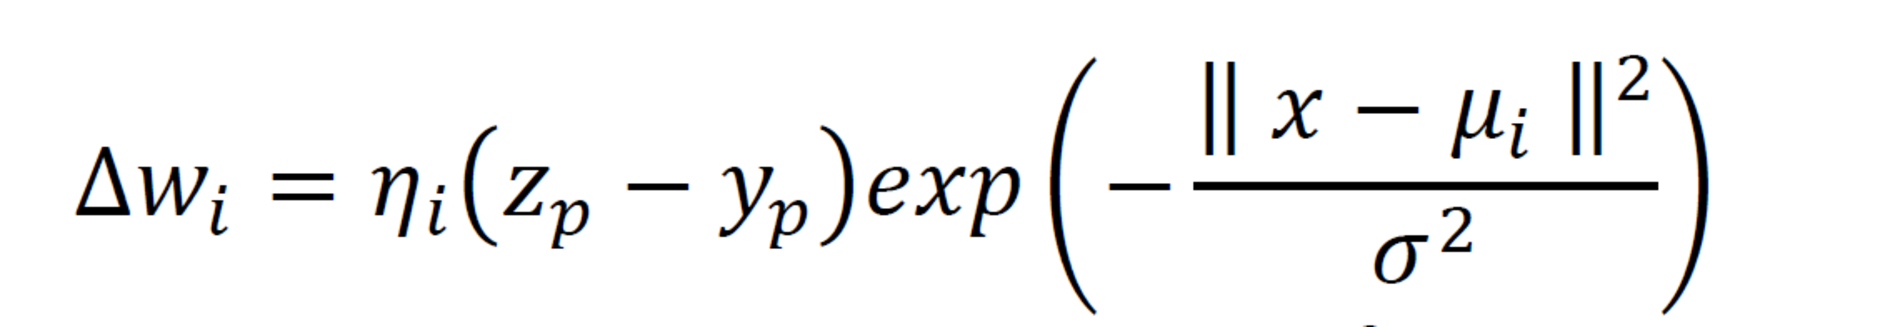
\includegraphics[width=2.5in]{eq1.pdf}
\caption{Variacion de los pesos $w_i$ }
\label{fig_cir}
\end{figure}
y para los centros quedaria como en la figura 4.6:\\
\begin{figure}
\centering
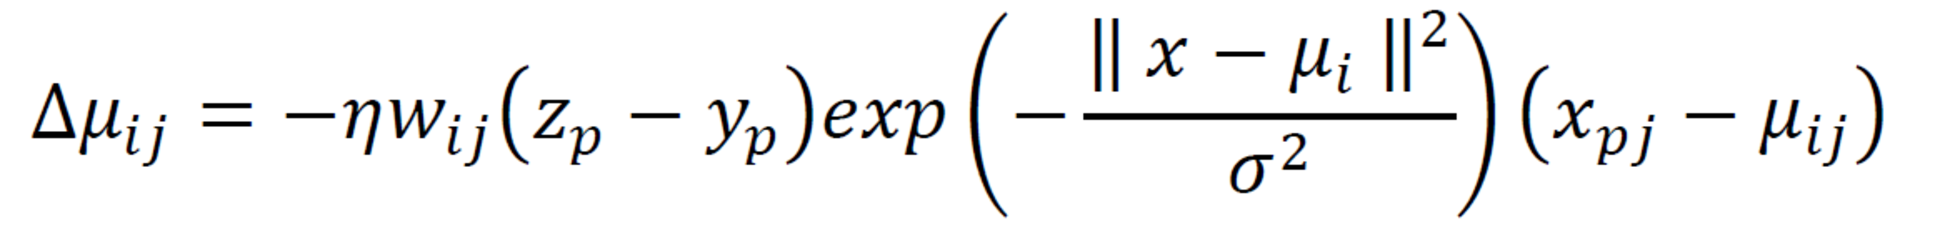
\includegraphics[width=2.5in]{eq2.pdf}
\caption{Variacion de los pesos $w_i$ }
\label{fig_cir}
\end{figure}

%
%Para este objetivo, utilizaremos el \textit{Neural Network Toolbox} de Matlab, el cual nos permite trabajar con multiples tipos de redes neuronales. En este caso hay  multiples clasificaciones de redes neuronales, las cuales pueden ser estaticas y dinamicas. Las estaticas (redes hacia adelante), no tienen retroalimentacion ni mucho menos delay(valores anteriores en el tiempo), en este tipo de redes neuronales las salidas solo dependen de la salida actual. En redes dinamic\'as la salida no solo depende de el valor actual$x_t$, sino que de valores anteriores $x_{t-1}$ , $x_{t-2}$ , $x_{t-3 }$..., de salidas anteriores, o estados en la red neuronal.\\
%Utilizaremos una red neuronal llamada \textit{Focused Time-Delay}, la cual es la red dinamica mas directa, que consiste en retroalimentaciones anteriores al actual valor. En este caso solo tendremos un neuron en nuestra red, la cual representa las orientaciones, esto porque se puede saber  hacia adonde ira el robot en el siguiente estado (resultado o salida de la red), esta red es muy util para prediccion de serie temporales (nuestro actual problema). Nuestra arquitectura es parecida a la figura 4.3:
%\begin{figure}
%\centering
%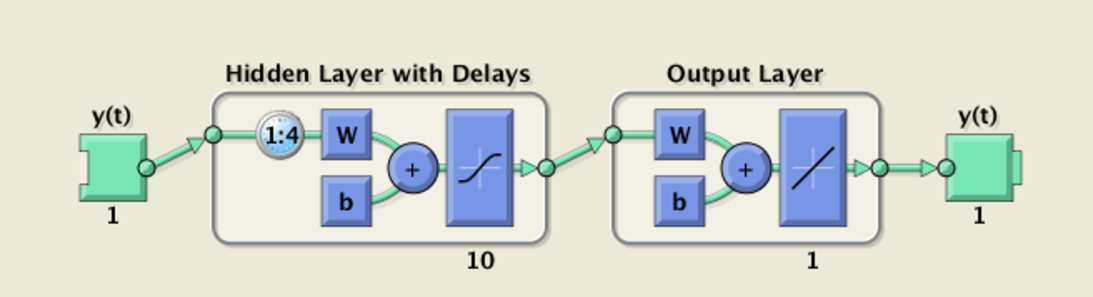
\includegraphics[width=2.5in]{red.pdf}
%\caption{Red Neuronal tipo Focused Time-Delay }
%\label{fig_cir}
%\end{figure}

